\graphicspath{{capitulos/Capitulo1-Introduccion/recursos/}}


\section{Introducción}

Este proyecto nace como continuación del proyecto ABACO, iniciado en 2015 por la Universidad Politécnica de Madrid en
colaboración con la empresa de innovación en el tráfico aéreo CRIDA\footnote{\url{https://crida.es}}, que pretende la
automatización del proceso de creación de la planificación de los turnos de los trabajadores que controlan el espacio aéreo.
\\

En ésta sección se describe el contexto principal y las hipótesis iniciales de las que parte el proyecto, así como una
ligera introducción al problema bajo estudio en el presente proyecto de fin de máster. Por su parte, en el
\refcruzada{Apartado}{apartado:2}, se describirá el problema en profundidad; el \refcruzada{Apartado}{apartado:3}
la metodología propuesta para su resolución; en el \refcruzada{Apartado}{apartado:4} los detalles de implementación;
en el \refcruzada{Apartado}{apartado:5} los resultados experimentales obtenidos; y, finalmente, en el
\refcruzada{Apartado}{apartado:6} las conclusiones y trabajo a futuro. También \NOTE{completar con los anexos} % TODO: Complemtar con los anexos
\\

El proyecto ABACO es realmente grande, y continua en constante evolución, pasando por las manos de diferentes alumnos
tanto de máster como de doctorado, cuyos trabajos se encuentran citados a lo largo de este documento. Por ello, este
trabajo pretende continuar el proyecto llevándolo un nivel más allá: hasta ahora el sistema resolvía unicamente el
problema de conformar por completo la distribución del personal, sin embargo, la empresa necesita en algunas ocasiones
reescribir parte de la planificación debido a una incidencia, por ejemplo la baja repentina de uno de los trabajadores,
por lo tanto éste nuevo problema consiste en resolver parte del problema, reescribiendo unicamente aquella parte de la
planificación que pertenezca al futuro, manteniendo lo anterior como constante. Por supuesto, para conformar la nueva
solución, se ha de considerar en todo momento la parte fija. El problema se describe en detalle en el \refcruzada{Apartado}{apartado:2}
\\

Además, debido a los requisitos del nuevo sistema, trataremos también de mejorar el rendimiento general del sistema,
modificando ciertas partes del software anterior para lograr mejor rendimiento.

\subsection{Objetivos del proyecto}

%\makeatletter
\label{sec:Objectivos}
\begin{enumerate}[label={H\arabic*}]
    \item[\namedlabel{H1}]  Es posible implementar las modificaciones y extensiones al sistema en un tiempo máximo
    \item de 7 meses, de forma que cumpla todos los requisitos del mismo y resuelva el problema dado %TODO referenciar el apartado de requisitos
    \item[\namedlabel{H2}]  El empleo de la metaheurística VNS mejora el rendimiento neto
    \footnote{Entiéndase como el coste computacional en unidades de tiempo aislado de la metaheurística, no del sistema en su totalidad}
    del sistema en comparación con el SA
    %\item[\namedlabel{H3}]  Custom item label for entry three
\end{enumerate}
%\makeatother


%\ref{item:H2}

%\begin{figure}
%	\centering
%	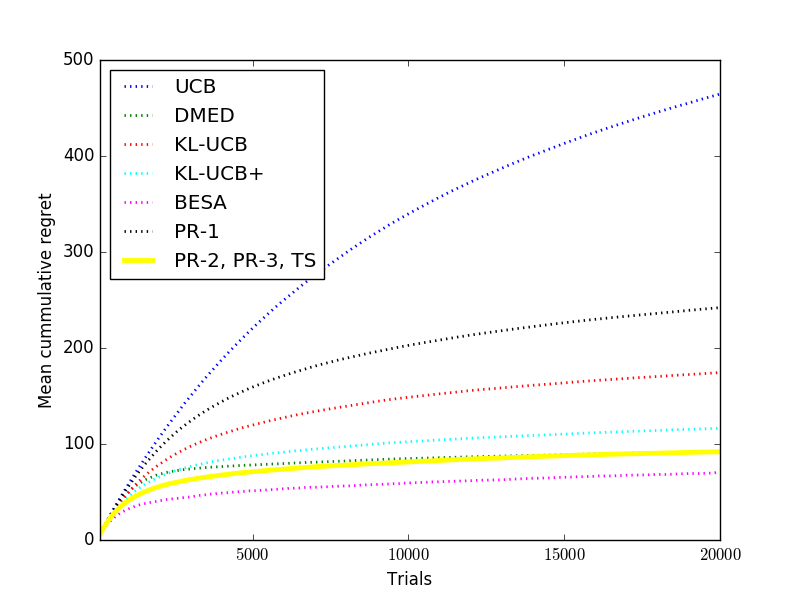
\includegraphics[width=0.7\linewidth]{Figure1a}
%	\caption{figura de test}
%	\label{fig:figure1a}
%\end{figure}

\subsection{Glosario}
\label{sec:Definiciones}
\begin{description}
    \item[ACC (Centro de Control)] \label{ACC}
    <<Centro de control de tránsito aéreo responsable de la circulación aérea segura a lo largo de las rutas ATS (servicio de tránsito aéreo). Un ACC se divide en varios sectores, cada uno de los cuales tiene claramente definidas sus responsabilidades. Los procedimientos para transferir una aeronave de un sector a otro entre estados limítrofes están perfectamente definidos por acuerdos internacionales, así como bilaterales>>.~\cite{ENAIRE-web}

    \item [ATC (Control de Tránsito Aéreo)] \label{ATC} <<Término común que designa todos los servicios proporcionados para asegurar y acelerar el flujo de tráfico aéreo a través del espacio aéreo controlado>>.~\cite{ENAIRE-web}

    \item [Núcleo] \label{Nucleo} Conjunto de Sectores. Un sector puede pertenecer a más de un núcleo (relación N a N). Esta agrupación se lleva a cabo para poder gestionar los posibles sectores que cada controlador puede controlar, de esta forma, un controlador tiene acreditación para un único núcleo.

    \item[\namedlabel{Matriz de Afinidad}] Tabla o matriz booleana cuyas filas y columnas son los diferentes sectores de una Unidad de Control dada, de forma que la intersección de dos sectores tendrá el valor de Cierto si y solo si los sectores son afines entre sí (relación bidireccional)

    \item[TMA] \label{TMA} Área de control terminal. <<Espacio aéreo controlado en torno a uno o varios aeropuertos donde se realizan las maniobras de aproximación (aterrizajes y despegues)>>~\cite{ENAIRE-web}.
\end{description}